\clearpage

\def\chaptertitle{Methodology}

\lhead{\emph{\chaptertitle}}

\chapter{\chaptertitle}
\label{ch:methodology}

Based on the overview of and challenges faced by edge computing paradigms in conforming to SLA constraints, the stated research questions, and the related works discussed above, a hybrid autoscaling algorithm to answer these questions was proposed during the course of this research project.\par

In this chapter, a brief discussion surrounding the problems and challenges of autoscaling edge architecture deployments in an SLA-compliant manner will be conducted in section \ref{sec:ch3-problem-overview}. Section \ref{sec:ch3-hybrid-autoscale-overview} will detail the high-level overview of the proposed hybrid autoscaler, the objectives of the algorithm, and the challenges it faces.

\section{Problem Overview}
\label{sec:ch3-problem-overview}

Edge architectures are split into three layers \cite{hamdan2020edge}. 
The cloud layer complements cloud-computing paradigms, wherein it manages the entire network architecture. The edge layer consists of data storage and communication with user devices. Finally, the device layer consists of all the user devices that will interact with the edge architecture.\par

The cloud layer has the most amount of resources allocated to it, as it is in charge of managing the entire network, and coordinating the resource allocation of the edge layer. However, the primary drawback is the distance between the user and the cloud layer results in significant latencies, making it unsuitable for storing user data. Thus only system critical applications such as the microservice control plane are deployed on this plane. The edge layer has far fewer resources than the cloud layer, but its proximity to the users results in lower network latency, making it ideal for resources scaling. For this reason, the edge layer consists of the microservice worker nodes. These nodes allocate resources dynamically according to user requirements through the process known as autoscaling.\par

The autoscaling should adhere to SLA metric, and try to minimize the number of violations. The SLA metric violation is defined as when it exceeds a certain threshold $\Delta$.
\[ metric_{SLA} < \Delta \]

The threshold $\Delta$ is typically split into three categories:
\begin{itemize}
    \item Flexible - This is typically the highest allowed metric for the application. Flexible SLA metrics are used to gauge the availability of the deployment. Most IoT applications employ this metric.
    \item Strict - This is the lowest allowed metric in the application. This metric is usually difficult to maintain, and is used by extremely time-critical applications such as tools for surgery.
    \item Moderate - This metric is a trade-off between flexible and strict SLA metrics. This metric is used by applications to ensure a real-time capability such as traffic light scheduling in railways.
\end{itemize}

The autoscaling will thus use a resource metric to scale its resources up or down. The autoscaler will check to see if the microservice metric exceeds the threshold for a certain time period, and if so, autoscale resources accordingly. A problem arises in the time it takes to scale these resources, however. This time to increase the number of resource replicas $\mathcal{R}$, known as cold start $\mathcal{C}(t)$ can be written as:

\[ \mathcal{C}(t) = \mathcal{R}_{download}(t) + \mathcal{R}_{deploy}(t) + \mathcal{R}_{register}(t)\]

The replica download time is usually a one-time delay due to optimizations done on modern container orchestration software. Thus, we can reduce this equation to the following:

\[ \mathcal{C}(t) \approx \mathcal{R}_{deploy}(t) + \mathcal{R}_{register}(t)\]

This time to deploy and register the replica to the container orchestration tool cannot be avoided. Furthermore, it can be shown that SLA violations $\mathcal{V} \propto \mathcal{C}(t)$ due to the correlation between cold-start delay and the lack of available resources.\par

Thus, when computing the SLA violation for a latency metric, the SLA violations can be re-written as the sum of the cold-start time and the round-trip time taken for the request.

\[ \mathcal{V} = \mathcal{C}(t) + req_{RT}(t)\]

This round-trip time is the combined sum of the inherent delay present in the network layer, and the time taken for the edge application to process the request.

\[ req_{RT}(t) = 2 \times latency_{N/W} + latency_{app} \]

The network delay can be reduced by investing in higher network bandwidths, but such improvements are out of scope of the project. Here we consider this latency to be a constant $\mathcal{K}$. Furthermore, $latency_{app}$ is proportional to the available resources to the application. Using this information, $req_{RT}(t)$ is approximated as:

\[ req_{RT}(t) \approx \mathcal{K} + resources_{app} \]

For horizontal pod autoscaling, the resource here are the pods $\mathcal{P}$ where $\mathcal{P} = \sum_{i} p_{i}$. These pods process the request. The final SLA equation can be re-written as follows:

\[ \mathcal{V} \propto ( \mathcal{C}(t) + \sum_{i} p_{i} )\]

Thus, the primary aim of the proactive autoscaler is to significantly reduce or even eliminate the cold start, while the reactive autoscaler aims to increase the number of resources assigned to the deployment.\par

A problem arises, however, in the amount of time and resources it takes to train a proactive model. Not only is a significant amount of CPU and memory resources consumed in the training process, but a large time-series data set is also required, without which the model will provide erroneous results until such time as the model is adequately trained. Hybrid models remove this constraint, but the questions regarding the model complexity remained an open issue.\par

Another issue in proactive autoscalers is that not only does it predict increases in utilization before-hand, it also does so for the drop-off in utilization. This can lead to the edge deployment prematurely reducing its resources, causing several SLA violations due to low availability of resources. To offset this, several hybrid algorithms combine the readings of their reactive and proactive autoscalers, and autoscale according to the highest reading. While this approach works, such predictions from the forecaster are redundant, and merely take up precious computation space in the edge deployment.\par

In most proactive autoscalers, the forecaster attempts to perfectly model the time-series curve to assign resources. Even in the hybrid algorithms that have been proposed in chapter \ref{ch:background}, the proactive sections of the autoscalers are generally unmodified proactive forecasters bundled together with a reactive component. This strategy of attempting to perfectly forecasting the curve is what takes such large amounts of resources.\par

In the autoscaler proposed in this thesis, the autoscaler will not attempt to predict the exact resource workload. Instead, the time-series graph is heavily simplified using a noise filtering method, and then inputted to the machine learning model. Furthermore, the LSTM only attempts to forecast the exact times when resource requirements starts to increase. Every other requirement, such as the stable resource utilization, as well as the drop-off in non-peak time periods can be handled by the reactive autoscaler, thus heavily simplifying the forecaster architecture. The simplified forecaster has an additional benefit in not requiring incredibly lengthy amounts of time-series data to be stored for it to make accurate predictions, thus this data can also be kept in the edge layer. This makes the autoscaler extremely lightweight and responsive, and thus capable of being deployed in an edge environment.\par

\section{Proposed Hybrid Autoscaler}
\label{sec:ch3-hybrid-autoscale-overview} 

\begin{figure}[htb]
    \centering
    \caption{Proposed hybrid architecture overview}
    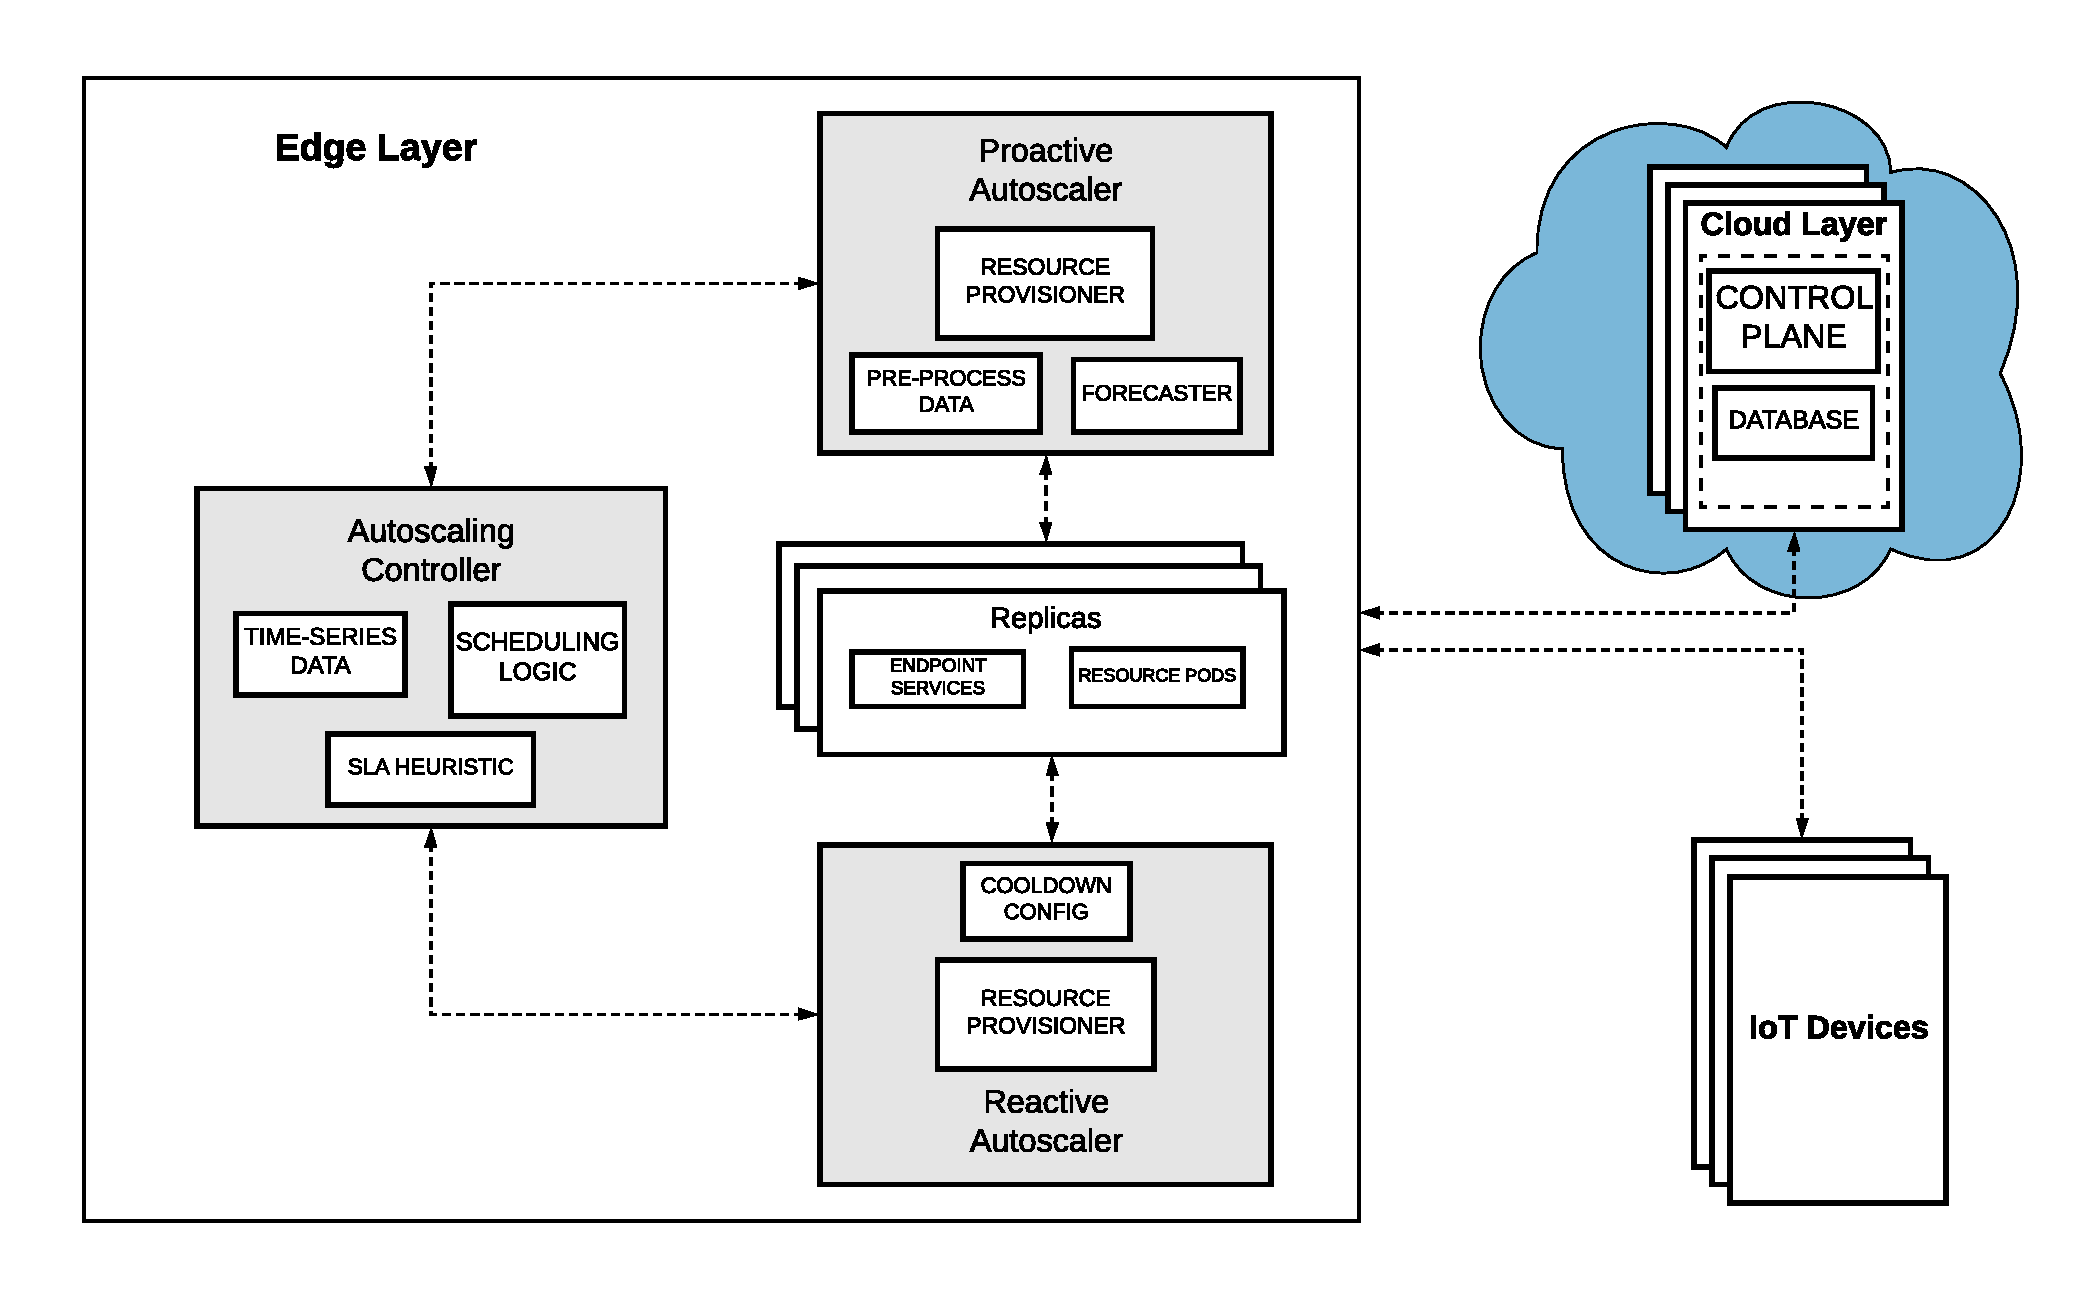
\includegraphics[width=1.0\linewidth]{Figures/Hybrid-Architecture-Overview.pdf}
    \label{fig:hybrid-arch-overview}
\end{figure}

An overview of the hybrid autoscaler architecture is shown in figure \ref{fig:hybrid-arch-overview}. The edge node consists of three main sections. The first is the reactive autoscaling section, which has the resource provisioner, and the configuration which dictates the cooldown logic for scaling up and down. As Zhang et al. \cite{zhang2019quantifying} demonstrated, the microservice system stability is directly related to the careful selection of cooldown parameters. Thus, these must be available to the user in a configuration setting.\par

\suhrid{TODO: Make sure to discuss the proactive autoscaler in detail in Ch4 using the notes written in Ch 2}
The second subsystem is the proactive autoscaler. A detailed breakdown of this will be discussed in chapter \ref{ch:experimental-setup}, however from a high-level perspective there are three main components. The resource provisioner is similar to that of the reactive autoscaler, however it also consists of a forecaster using machine learning techniques, and a data pre-processing algorithm. This algorithm removes any noise present in the time series data, and smoothens the graph, making it easier for the forecaster to make predictions in a low-cost manner.\par

Finally, the autoscaling daemon controls which autoscaling logic will be applied to the replicas, and also keeps a track of any SLA violations. It also hosts the time-series metric data, and has a feedback loop with the proactive autoscaler. If it detects any SLA violations caused after autoscaling, it adjusts the hyperparameters of the proactive forecaster automatically to attempt to predict the time-series in a more accurate manner. Correspondingly, a lack of SLA violations during a specific time period reverts the autoscaler parameters to attempt to streamline the training process further. Such a heuristic method allows for the freeing up of the complex hyperparameter tuning process seen in most proactive models. This is a key part of the architecture which is essential in answering one of the research questions outlined in the thesis.\par